\newcommand{\rev}{01 - 23-Jul-2021}
% REV01 Fri 23 Jul 2021 16:51:45 WIB
% START Fri 26 Mar 2021 12:10:02 WIB

\documentclass[12pt]{book}
\usepackage[a4paper, margin=50pt]{geometry}
\usepackage{colortbl}
\usepackage[hidelinks]{hyperref}
\usepackage[pdftex]{graphicx}

% Should be loaded after the hyperref and bookmark packages
\usepackage{chngcntr}
\counterwithin*{chapter}{part}
% \counterwithout{chapter}{part}

\newcommand{\pengarangs}{%
    Dickens McCartney\\
}
\newcommand{\judul}{%
Jenny Wren\\[13pt]
Our Mutual Friend
}

\begin{document}

\begin{titlepage}
    \begin{center}    

    \vspace*{15mm}
    \textbf{\Large \judul}

    \vspace*{30mm}       
    \textbf{by}

    \vspace*{15mm}    
    \textbf{\Large \pengarangs}

    \vspace*{4.0cm}

    \begin{center}
        
\includegraphics[width=40mm]{ucls-coat}
    \end{center}

    \textbf{
       Universe Centra Le Sahara (UCLS)\\[10pt]
       Omar Bakry School of Management\\[10pt]
       Jabal Acacus Campus, Ghat. \\[10pt]
       \url{https://jennywren.vlsm.org/} \\[10pt]
       Rev. \rev%
    }

    %\vspace*{5mm}    
    %\textbf{\LARGE \textcolor{red}{***** Work In Progress *****}}

    \end{center}

\end{titlepage}

\pagenumbering{roman}

\tableofcontents

\newpage

\chapter*{Jenny Wren}
\addcontentsline{toc}{chapter}{Jenny Wren}

\begin{verbatim}
Like so many girls
Jenny Wren could sing
But a broken heart
Took her soul away

Like the other girls
Jenny Wren took wing
She could see the world
And it's foolish ways

How, we, spend our days
Casting, love aside
Loosing, site of life
Day, by, day

She saw poverty
Breaking all the home
Wounded warriors
Took her song away

But the day will come
Jenny Wren will sing
When this broken world
Mends its foolish ways

Now we, spend our days
Catching, up on life
All because of you
Jenny Wren

--- Dickens McCartney
\end{verbatim}

\noindent
Jenny Wren lyrics \copyright MPL Communications Ltd. See also \url{https://jennywren.vlsm.org/}.
\newpage

\noindent
Jenny Wren --- whose real name is Fanny Cleaver,
is ''the dolls' dressmaker'' with whom Lizzie lives after her father dies.
She is crippled with a bad back, although not ugly.
She is very motherly towards her drunken father, whom she calls her ''bad child''.
Jenny later cares for Eugene while he recovers from Headstone's attack on his life.
She may have a romance with Sloppy at the end of the book,
which the reader may surmise will end in marriage.
Although her mannerisms give her a certain ''strangeness'', Jenny is very perceptive,
identifying Eugene Wrayburn's intentions towards Lizzie in his small actions.
Her role is a creator and a caretaker, 
and her ''pleasant fancies'' of ''flowers, bird song, numbers of blessed, 
white-clad children'' reflect the mind's ability to rise above adverse 
circumstances --- \url{https://en.wikipedia.org/wiki/Jenny_Wren}
\\[1pt]

\noindent
Jenny Wren aka Fanny Cleaver --- Sharp and sassy maker of doll's clothes, 
pincushions, and pen-wipers. 
Crippled (my back’s bad, and my legs are queer),
she lives with her drunken father whom she refers to as her bad child.
Lizzie Hexam, after the death of her father,
takes lodging with Jenny who helps Lizzie escape London when pursued by Bradley Headstone and Eugene Wrayburn.
It was difficult to guess the age of this strange creature,
for her poor figure furnished no clue to it,
and her face was at once so young and so old. Twelve,
or at the most thirteen, might be near the mark --- 
\url{https://www.charlesdickenspage.com/dickens-characters-t-z.html}
\\[1pt]

\noindent
=== Rev. \rev ===

\newpage

\pagenumbering{arabic}

\part{Book the First:\\THE CUP AND THE LIP}
% REV02 Fri 23 Jul 2021 17:19:30 WIB
% REV01 Sun 28 Mar 2021 09:52:23 WIB
% START Fri 26 Mar 2021 17:22:59 WIB

\chapter{ON THE LOOK OUT}

In these times of ours, though concerning the exact year there is no
need to be precise, a boat of dirty and disreputable appearance,
with two figures in it, floated on the Thames, between Southwark
bridge which is of iron, and London Bridge which is of stone, as an
autumn evening was closing in.

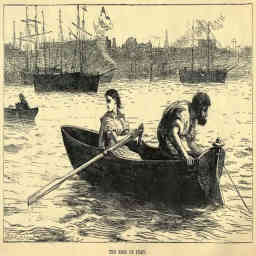
\includegraphics[scale=2.3]{01-01-01}

The figures in this boat were those of a strong man with ragged
grizzled hair and a sun-browned face, and a dark girl of nineteen or
twenty, sufficiently like him to be recognizable as his daughter.
The girl rowed, pulling a pair of sculls very easily; the man, with
the rudder-lines slack in his hands, and his hands loose in his
waistband, kept an eager look out. He had no net, hook, or line,
and he could not be a fisherman; his boat had no cushion for a
sitter, no paint, no inscription, no appliance beyond a rusty
boathook and a coil of rope, and he could not be a waterman; his
boat was too crazy and too small to take in cargo for delivery, and
he could not be a lighterman or river-carrier; there was no clue to
what he looked for, but he looked for something, with a most intent
and searching gaze. The tide, which had turned an hour before,
was running down, and his eyes watched every little race and eddy
in its broad sweep, as the boat made slight head-way against it, or
drove stern foremost before it, according as he directed his
daughter by a movement of his head. She watched his face as
earnestly as he watched the river. But, in the intensity of her look
there was a touch of dread or horror.


\part{Book The Second:\\BIRDS OF A FEATHER}
% REV01 Tue 22 Jun 2021 12:31:50 WIB
% START Tue 04 May 2021 13:55:16 WIB

\chapter{OF AN EDUCATIONAL CHARACTER}

The school at which young Charley Hexam had first learned from a
book--the streets being, for pupils of his degree, the great Preparatory
Establishment in which very much that is never unlearned is learned
without and before book--was a miserable loft in an unsavoury yard. Its
atmosphere was oppressive and disagreeable; it was crowded, noisy,
and confusing; half the pupils dropped asleep, or fell into a state of
waking stupefaction; the other half kept them in either condition by
maintaining a monotonous droning noise, as if they were performing, out
of time and tune, on a ruder sort of bagpipe. The teachers, animated
solely by good intentions, had no idea of execution, and a lamentable
jumble was the upshot of their kind endeavours.

It was a school for all ages, and for both sexes. The latter were kept
apart, and the former were partitioned off into square assortments. But,
all the place was pervaded by a grimly ludicrous pretence that every
pupil was childish and innocent. This pretence, much favoured by the
lady-visitors, led to the ghastliest absurdities. Young women old in
the vices of the commonest and worst life, were expected to profess
themselves enthralled by the good child’s book, the Adventures of
Little Margery, who resided in the village cottage by the mill; severely
reproved and morally squashed the miller, when she was five and he was
fifty; divided her porridge with singing birds; denied herself a new
nankeen bonnet, on the ground that the turnips did not wear nankeen
bonnets, neither did the sheep who ate them; who plaited straw and
delivered the dreariest orations to all comers, at all sorts of
unseasonable times. So, unwieldy young dredgers and hulking mudlarks
were referred to the experiences of Thomas Twopence, who, having
resolved not to rob (under circumstances of uncommon atrocity) his
particular friend and benefactor, of eighteenpence, presently came into
supernatural possession of three and sixpence, and lived a shining light
ever afterwards. (Note, that the benefactor came to no good.) Several
swaggering sinners had written their own biographies in the same strain;
it always appearing from the lessons of those very boastful persons,
that you were to do good, not because it WAS good, but because you were
to make a good thing of it. Contrariwise, the adult pupils were taught
to read (if they could learn) out of the New Testament; and by dint of
stumbling over the syllables and keeping their bewildered eyes on the
particular syllables coming round to their turn, were as absolutely
ignorant of the sublime history, as if they had never seen or heard of
it. An exceedingly and confoundingly perplexing jumble of a school,
in fact, where black spirits and grey, red spirits and white, jumbled
jumbled jumbled jumbled, jumbled every night. And particularly every
Sunday night. For then, an inclined plane of unfortunate infants would
be handed over to the prosiest and worst of all the teachers with good
intentions, whom nobody older would endure. Who, taking his stand on
the floor before them as chief executioner, would be attended by a
conventional volunteer boy as executioner’s assistant. When and where it
first became the conventional system that a weary or inattentive infant
in a class must have its face smoothed downward with a hot hand, or when
and where the conventional volunteer boy first beheld such system in
operation, and became inflamed with a sacred zeal to administer it,
matters not. It was the function of the chief executioner to hold forth,
and it was the function of the acolyte to dart at sleeping infants,
yawning infants, restless infants, whimpering infants, and smooth their
wretched faces; sometimes with one hand, as if he were anointing them
for a whisker; sometimes with both hands, applied after the fashion of
blinkers. And so the jumble would be in action in this department for a
mortal hour; the exponent drawling on to My Dearert Childerrenerr, let
us say, for example, about the beautiful coming to the Sepulchre; and
repeating the word Sepulchre (commonly used among infants) five hundred
times, and never once hinting what it meant; the conventional boy
smoothing away right and left, as an infallible commentary; the whole
hot-bed of flushed and exhausted infants exchanging measles, rashes,
whooping-cough, fever, and stomach disorders, as if they were assembled
in High Market for the purpose.

Even in this temple of good intentions, an exceptionally sharp boy
exceptionally determined to learn, could learn something, and, having
learned it, could impart it much better than the teachers; as being
more knowing than they, and not at the disadvantage in which they stood
towards the shrewder pupils. In this way it had come about that Charley
Hexam had risen in the jumble, taught in the jumble, and been received
from the jumble into a better school.

‘So you want to go and see your sister, Hexam?’

‘If you please, Mr Headstone.’

‘I have half a mind to go with you. Where does your sister live?’

‘Why, she is not settled yet, Mr Headstone. I’d rather you didn’t see
her till she is settled, if it was all the same to you.’

‘Look here, Hexam.’ Mr Bradley Headstone, highly certificated
stipendiary schoolmaster, drew his right forefinger through one of the
buttonholes of the boy’s coat, and looked at it attentively. ‘I hope
your sister may be good company for you?’

‘Why do you doubt it, Mr Headstone?’

‘I did not say I doubted it.’

‘No, sir; you didn’t say so.’

Bradley Headstone looked at his finger again, took it out of the
buttonhole and looked at it closer, bit the side of it and looked at it
again.

‘You see, Hexam, you will be one of us. In good time you are sure to
pass a creditable examination and become one of us. Then the question
is--’

The boy waited so long for the question, while the schoolmaster looked
at a new side of his finger, and bit it, and looked at it again, that at
length the boy repeated:

‘The question is, sir--?’

‘Whether you had not better leave well alone.’

‘Is it well to leave my sister alone, Mr Headstone?’

‘I do not say so, because I do not know. I put it to you. I ask you to
think of it. I want you to consider. You know how well you are doing
here.’

‘After all, she got me here,’ said the boy, with a struggle.

‘Perceiving the necessity of it,’ acquiesced the schoolmaster, ‘and
making up her mind fully to the separation. Yes.’

The boy, with a return of that former reluctance or struggle or whatever
it was, seemed to debate with himself. At length he said, raising his
eyes to the master’s face:

‘I wish you’d come with me and see her, Mr Headstone, though she is not
settled. I wish you’d come with me, and take her in the rough, and judge
her for yourself.’

‘You are sure you would not like,’ asked the schoolmaster, ‘to prepare
her?’

‘My sister Lizzie,’ said the boy, proudly, ‘wants no preparing, Mr
Headstone. What she is, she is, and shows herself to be. There’s no
pretending about my sister.’

His confidence in her, sat more easily upon him than the indecision with
which he had twice contended. It was his better nature to be true to
her, if it were his worse nature to be wholly selfish. And as yet the
better nature had the stronger hold.

‘Well, I can spare the evening,’ said the schoolmaster. ‘I am ready to
walk with you.’

‘Thank you, Mr Headstone. And I am ready to go.’

Bradley Headstone, in his decent black coat and waistcoat, and decent
white shirt, and decent formal black tie, and decent pantaloons of
pepper and salt, with his decent silver watch in his pocket and its
decent hair-guard round his neck, looked a thoroughly decent young man
of six-and-twenty. He was never seen in any other dress, and yet there
was a certain stiffness in his manner of wearing this, as if there were
a want of adaptation between him and it, recalling some mechanics in
their holiday clothes. He had acquired mechanically a great store of
teacher’s knowledge. He could do mental arithmetic mechanically, sing
at sight mechanically, blow various wind instruments mechanically, even
play the great church organ mechanically. From his early childhood up,
his mind had been a place of mechanical stowage. The arrangement of
his wholesale warehouse, so that it might be always ready to meet the
demands of retail dealers history here, geography there, astronomy to
the right, political economy to the left--natural history, the physical
sciences, figures, music, the lower mathematics, and what not, all in
their several places--this care had imparted to his countenance a look
of care; while the habit of questioning and being questioned had given
him a suspicious manner, or a manner that would be better described as
one of lying in wait. There was a kind of settled trouble in the face.
It was the face belonging to a naturally slow or inattentive intellect
that had toiled hard to get what it had won, and that had to hold it now
that it was gotten. He always seemed to be uneasy lest anything should
be missing from his mental warehouse, and taking stock to assure
himself.

Suppression of so much to make room for so much, had given him a
constrained manner, over and above. Yet there was enough of what was
animal, and of what was fiery (though smouldering), still visible in
him, to suggest that if young Bradley Headstone, when a pauper lad, had
chanced to be told off for the sea, he would not have been the last man
in a ship’s crew. Regarding that origin of his, he was proud, moody, and
sullen, desiring it to be forgotten. And few people knew of it.

In some visits to the Jumble his attention had been attracted to this
boy Hexam. An undeniable boy for a pupil-teacher; an undeniable boy
to do credit to the master who should bring him on. Combined with this
consideration, there may have been some thought of the pauper lad now
never to be mentioned. Be that how it might, he had with pains gradually
worked the boy into his own school, and procured him some offices to
discharge there, which were repaid with food and lodging. Such were the
circumstances that had brought together, Bradley Headstone and young
Charley Hexam that autumn evening. Autumn, because full half a year had
come and gone since the bird of prey lay dead upon the river-shore.

The schools--for they were twofold, as the sexes--were down in that
district of the flat country tending to the Thames, where Kent and
Surrey meet, and where the railways still bestride the market-gardens
that will soon die under them. The schools were newly built, and there
were so many like them all over the country, that one might have thought
the whole were but one restless edifice with the locomotive gift of
Aladdin’s palace. They were in a neighbourhood which looked like a toy
neighbourhood taken in blocks out of a box by a child of particularly
incoherent mind, and set up anyhow; here, one side of a new street;
there, a large solitary public-house facing nowhere; here, another
unfinished street already in ruins; there, a church; here, an immense
new warehouse; there, a dilapidated old country villa; then, a medley
of black ditch, sparkling cucumber-frame, rank field, richly cultivated
kitchen-garden, brick viaduct, arch-spanned canal, and disorder of
frowziness and fog. As if the child had given the table a kick, and gone
to sleep.

But, even among school-buildings, school-teachers, and school-pupils,
all according to pattern and all engendered in the light of the latest
Gospel according to Monotony, the older pattern into which so many
fortunes have been shaped for good and evil, comes out. It came out in
Miss Peecher the schoolmistress, watering her flowers, as Mr Bradley
Headstone walked forth. It came out in Miss Peecher the schoolmistress,
watering the flowers in the little dusty bit of garden attached to her
small official residence, with little windows like the eyes in needles,
and little doors like the covers of school-books.

Small, shining, neat, methodical, and buxom was Miss Peecher;
cherry-cheeked and tuneful of voice. A little pincushion, a little
housewife, a little book, a little workbox, a little set of tables and
weights and measures, and a little woman, all in one. She could write
a little essay on any subject, exactly a slate long, beginning at the
left-hand top of one side and ending at the right-hand bottom of the
other, and the essay should be strictly according to rule. If Mr Bradley
Headstone had addressed a written proposal of marriage to her, she would
probably have replied in a complete little essay on the theme exactly a
slate long, but would certainly have replied Yes. For she loved him. The
decent hair-guard that went round his neck and took care of his decent
silver watch was an object of envy to her. So would Miss Peecher have
gone round his neck and taken care of him. Of him, insensible. Because
he did not love Miss Peecher.

Miss Peecher’s favourite pupil, who assisted her in her little
household, was in attendance with a can of water to replenish her little
watering-pot, and sufficiently divined the state of Miss Peecher’s
affections to feel it necessary that she herself should love young
Charley Hexam. So, there was a double palpitation among the double
stocks and double wall-flowers, when the master and the boy looked over
the little gate.

‘A fine evening, Miss Peecher,’ said the Master.

‘A very fine evening, Mr Headstone,’ said Miss Peecher. ‘Are you taking
a walk?’

‘Hexam and I are going to take a long walk.’

‘Charming weather,’ remarked Miss Peecher, ‘FOR a long walk.’

‘Ours is rather on business than mere pleasure,’ said the Master. Miss
Peecher inverting her watering-pot, and very carefully shaking out the
few last drops over a flower, as if there were some special virtue in
them which would make it a Jack’s beanstalk before morning, called for
replenishment to her pupil, who had been speaking to the boy.

‘Good-night, Miss Peecher,’ said the Master.

‘Good-night, Mr Headstone,’ said the Mistress.

The pupil had been, in her state of pupilage, so imbued with the
class-custom of stretching out an arm, as if to hail a cab or omnibus,
whenever she found she had an observation on hand to offer to Miss
Peecher, that she often did it in their domestic relations; and she did
it now.

‘Well, Mary Anne?’ said Miss Peecher.

‘If you please, ma’am, Hexam said they were going to see his sister.’

‘But that can’t be, I think,’ returned Miss Peecher: ‘because Mr
Headstone can have no business with HER.’

Mary Anne again hailed.

‘Well, Mary Anne?’

‘If you please, ma’am, perhaps it’s Hexam’s business?’

‘That may be,’ said Miss Peecher. ‘I didn’t think of that. Not that it
matters at all.’

Mary Anne again hailed.

‘Well, Mary Anne?’

‘They say she’s very handsome.’

‘Oh, Mary Anne, Mary Anne!’ returned Miss Peecher, slightly colouring
and shaking her head, a little out of humour; ‘how often have I told you
not to use that vague expression, not to speak in that general way? When
you say THEY say, what do you mean? Part of speech They?’

Mary Anne hooked her right arm behind her in her left hand, as being
under examination, and replied:

‘Personal pronoun.’

‘Person, They?’

‘Third person.’

‘Number, They?’

‘Plural number.’

‘Then how many do you mean, Mary Anne? Two? Or more?’

‘I beg your pardon, ma’am,’ said Mary Anne, disconcerted now she came
to think of it; ‘but I don’t know that I mean more than her brother
himself.’ As she said it, she unhooked her arm.

‘I felt convinced of it,’ returned Miss Peecher, smiling again. ‘Now
pray, Mary Anne, be careful another time. He says is very different from
they say, remember. Difference between he says and they say? Give it
me.’

Mary Anne immediately hooked her right arm behind her in her left
hand--an attitude absolutely necessary to the situation--and replied:
‘One is indicative mood, present tense, third person singular, verb
active to say. Other is indicative mood, present tense, third person
plural, verb active to say.’

‘Why verb active, Mary Anne?’

‘Because it takes a pronoun after it in the objective case, Miss
Peecher.’

‘Very good indeed,’ remarked Miss Peecher, with encouragement. ‘In fact,
could not be better. Don’t forget to apply it, another time, Mary Anne.’
This said, Miss Peecher finished the watering of her flowers, and
went into her little official residence, and took a refresher of the
principal rivers and mountains of the world, their breadths, depths, and
heights, before settling the measurements of the body of a dress for her
own personal occupation.

Bradley Headstone and Charley Hexam duly got to the Surrey side of
Westminster Bridge, and crossed the bridge, and made along the Middlesex
shore towards Millbank. In this region are a certain little street
called Church Street, and a certain little blind square, called Smith
Square, in the centre of which last retreat is a very hideous church
with four towers at the four corners, generally resembling some
petrified monster, frightful and gigantic, on its back with its legs
in the air. They found a tree near by in a corner, and a blacksmith’s
forge, and a timber yard, and a dealer’s in old iron. What a rusty
portion of a boiler and a great iron wheel or so meant by lying
half-buried in the dealer’s fore-court, nobody seemed to know or to want
to know. Like the Miller of questionable jollity in the song, They cared
for Nobody, no not they, and Nobody cared for them.

After making the round of this place, and noting that there was a deadly
kind of repose on it, more as though it had taken laudanum than fallen
into a natural rest, they stopped at the point where the street and the
square joined, and where there were some little quiet houses in a row.
To these Charley Hexam finally led the way, and at one of these stopped.

‘This must be where my sister lives, sir. This is where she came for a
temporary lodging, soon after father’s death.’

‘How often have you seen her since?’

‘Why, only twice, sir,’ returned the boy, with his former reluctance;
‘but that’s as much her doing as mine.’

‘How does she support herself?’

‘She was always a fair needlewoman, and she keeps the stockroom of a
seaman’s outfitter.’

‘Does she ever work at her own lodging here?’

‘Sometimes; but her regular hours and regular occupation are at their
place of business, I believe, sir. This is the number.’

The boy knocked at a door, and the door promptly opened with a spring
and a click. A parlour door within a small entry stood open, and
disclosed a child--a dwarf--a girl--a something--sitting on a little low
old-fashioned arm-chair, which had a kind of little working bench before
it.

‘I can’t get up,’ said the child, ‘because my back’s bad, and my legs
are queer. But I’m the person of the house.’

‘Who else is at home?’ asked Charley Hexam, staring.

‘Nobody’s at home at present,’ returned the child, with a glib assertion
of her dignity, ‘except the person of the house. What did you want,
young man?’

‘I wanted to see my sister.’

‘Many young men have sisters,’ returned the child. ‘Give me your name,
young man?’

The queer little figure, and the queer but not ugly little face, with
its bright grey eyes, were so sharp, that the sharpness of the manner
seemed unavoidable. As if, being turned out of that mould, it must be
sharp.

‘Hexam is my name.’

‘Ah, indeed?’ said the person of the house. ‘I thought it might be. Your
sister will be in, in about a quarter of an hour. I am very fond of your
sister. She’s my particular friend. Take a seat. And this gentleman’s
name?’

‘Mr Headstone, my schoolmaster.’

‘Take a seat. And would you please to shut the street door first? I
can’t very well do it myself; because my back’s so bad, and my legs are
so queer.’

They complied in silence, and the little figure went on with its work of
gumming or gluing together with a camel’s-hair brush certain pieces
of cardboard and thin wood, previously cut into various shapes. The
scissors and knives upon the bench showed that the child herself had cut
them; and the bright scraps of velvet and silk and ribbon also strewn
upon the bench showed that when duly stuffed (and stuffing too was
there), she was to cover them smartly. The dexterity of her nimble
fingers was remarkable, and, as she brought two thin edges accurately
together by giving them a little bite, she would glance at the visitors
out of the corners of her grey eyes with a look that out-sharpened all
her other sharpness.

‘You can’t tell me the name of my trade, I’ll be bound,’ she said, after
taking several of these observations.

‘You make pincushions,’ said Charley.

‘What else do I make?’

‘Pen-wipers,’ said Bradley Headstone.

‘Ha! ha! What else do I make? You’re a schoolmaster, but you can’t tell
me.’

‘You do something,’ he returned, pointing to a corner of the little
bench, ‘with straw; but I don’t know what.’

‘Well done you!’ cried the person of the house. ‘I only make pincushions
and pen-wipers, to use up my waste. But my straw really does belong to
my business. Try again. What do I make with my straw?’

‘Dinner-mats?’

‘A schoolmaster, and says dinner-mats! I’ll give you a clue to my trade,
in a game of forfeits. I love my love with a B because she’s Beautiful;
I hate my love with a B because she is Brazen; I took her to the sign of
the Blue Boar, and I treated her with Bonnets; her name’s Bouncer, and
she lives in Bedlam.--Now, what do I make with my straw?’

‘Ladies’ bonnets?’

‘Fine ladies’,’ said the person of the house, nodding assent. ‘Dolls’.
I’m a Doll’s Dressmaker.’

‘I hope it’s a good business?’

The person of the house shrugged her shoulders and shook her head. ‘No.
Poorly paid. And I’m often so pressed for time! I had a doll married,
last week, and was obliged to work all night. And it’s not good for me,
on account of my back being so bad and my legs so queer.’

They looked at the little creature with a wonder that did not diminish,
and the schoolmaster said: ‘I am sorry your fine ladies are so
inconsiderate.’

‘It’s the way with them,’ said the person of the house, shrugging her
shoulders again. ‘And they take no care of their clothes, and they
never keep to the same fashions a month. I work for a doll with three
daughters. Bless you, she’s enough to ruin her husband!’ The person of
the house gave a weird little laugh here, and gave them another look out
of the corners of her eyes. She had an elfin chin that was capable of
great expression; and whenever she gave this look, she hitched this chin
up. As if her eyes and her chin worked together on the same wires.

‘Are you always as busy as you are now?’

‘Busier. I’m slack just now. I finished a large mourning order the day
before yesterday. Doll I work for, lost a canary-bird.’ The person of
the house gave another little laugh, and then nodded her head several
times, as who should moralize, ‘Oh this world, this world!’

‘Are you alone all day?’ asked Bradley Headstone. ‘Don’t any of the
neighbouring children--?’

‘Ah, lud!’ cried the person of the house, with a little scream, as
if the word had pricked her. ‘Don’t talk of children. I can’t bear
children. I know their tricks and their manners.’ She said this with an
angry little shake of her tight fist close before her eyes.

Perhaps it scarcely required the teacher-habit, to perceive that the
doll’s dressmaker was inclined to be bitter on the difference between
herself and other children. But both master and pupil understood it so.

‘Always running about and screeching, always playing and fighting,
always skip-skip-skipping on the pavement and chalking it for their
games! Oh! I know their tricks and their manners!’ Shaking the little
fist as before. ‘And that’s not all. Ever so often calling names in
through a person’s keyhole, and imitating a person’s back and legs. Oh!
I know their tricks and their manners. And I’ll tell you what I’d do, to
punish ‘em. There’s doors under the church in the Square--black doors,
leading into black vaults. Well! I’d open one of those doors, and I’d
cram ‘em all in, and then I’d lock the door and through the keyhole I’d
blow in pepper.’

‘What would be the good of blowing in pepper?’ asked Charley Hexam.

‘To set ‘em sneezing,’ said the person of the house, ‘and make their
eyes water. And when they were all sneezing and inflamed, I’d mock ‘em
through the keyhole. Just as they, with their tricks and their manners,
mock a person through a person’s keyhole!’

An uncommonly emphatic shake of her little fist close before her eyes,
seemed to ease the mind of the person of the house; for she added
with recovered composure, ‘No, no, no. No children for me. Give me
grown-ups.’

It was difficult to guess the age of this strange creature, for her poor
figure furnished no clue to it, and her face was at once so young and so
old. Twelve, or at the most thirteen, might be near the mark.

‘I always did like grown-ups,’ she went on, ‘and always kept company
with them. So sensible. Sit so quiet. Don’t go prancing and capering
about! And I mean always to keep among none but grown-ups till I marry.
I suppose I must make up my mind to marry, one of these days.’

She listened to a step outside that caught her ear, and there was a soft
knock at the door. Pulling at a handle within her reach, she said,
with a pleased laugh: ‘Now here, for instance, is a grown-up that’s my
particular friend!’ and Lizzie Hexam in a black dress entered the room.

‘Charley! You!’

Taking him to her arms in the old way--of which he seemed a little
ashamed--she saw no one else.

‘There, there, there, Liz, all right my dear. See! Here’s Mr Headstone
come with me.’

Her eyes met those of the schoolmaster, who had evidently expected
to see a very different sort of person, and a murmured word or two
of salutation passed between them. She was a little flurried by the
unexpected visit, and the schoolmaster was not at his ease. But he never
was, quite.

‘I told Mr Headstone you were not settled, Liz, but he was so kind as to
take an interest in coming, and so I brought him. How well you look!’

Bradley seemed to think so.

‘Ah! Don’t she, don’t she?’ cried the person of the house, resuming her
occupation, though the twilight was falling fast. ‘I believe you she
does! But go on with your chat, one and all:

\begin{verbatim}
     You one two three,
     My com-pa-nie,
     And don’t mind me.’
\end{verbatim}

--pointing this impromptu rhyme with three points of her thin
fore-finger.

‘I didn’t expect a visit from you, Charley,’ said his sister. ‘I
supposed that if you wanted to see me you would have sent to me,
appointing me to come somewhere near the school, as I did last time.
I saw my brother near the school, sir,’ to Bradley Headstone, ‘because
it’s easier for me to go there, than for him to come here. I work about
midway between the two places.’

‘You don’t see much of one another,’ said Bradley, not improving in
respect of ease.

‘No.’ With a rather sad shake of her head. ‘Charley always does well, Mr
Headstone?’

‘He could not do better. I regard his course as quite plain before him.’

‘I hoped so. I am so thankful. So well done of you, Charley dear! It is
better for me not to come (except when he wants me) between him and his
prospects. You think so, Mr Headstone?’

Conscious that his pupil-teacher was looking for his answer, that he
himself had suggested the boy’s keeping aloof from this sister, now seen
for the first time face to face, Bradley Headstone stammered:

‘Your brother is very much occupied, you know. He has to work hard. One
cannot but say that the less his attention is diverted from his work,
the better for his future. When he shall have established himself, why
then--it will be another thing then.’

Lizzie shook her head again, and returned, with a quiet smile: ‘I always
advised him as you advise him. Did I not, Charley?’

‘Well, never mind that now,’ said the boy. ‘How are you getting on?’

‘Very well, Charley. I want for nothing.’

‘You have your own room here?’

‘Oh yes. Upstairs. And it’s quiet, and pleasant, and airy.’

‘And she always has the use of this room for visitors,’ said the
person of the house, screwing up one of her little bony fists, like an
opera-glass, and looking through it, with her eyes and her chin in that
quaint accordance. ‘Always this room for visitors; haven’t you, Lizzie
dear?’

It happened that Bradley Headstone noticed a very slight action of
Lizzie Hexam’s hand, as though it checked the doll’s dressmaker. And it
happened that the latter noticed him in the same instant; for she made
a double eyeglass of her two hands, looked at him through it, and cried,
with a waggish shake of her head: ‘Aha! Caught you spying, did I?’

It might have fallen out so, any way; but Bradley Headstone also noticed
that immediately after this, Lizzie, who had not taken off her bonnet,
rather hurriedly proposed that as the room was getting dark they should
go out into the air. They went out; the visitors saying good-night to
the doll’s dressmaker, whom they left, leaning back in her chair with
her arms crossed, singing to herself in a sweet thoughtful little voice.

‘I’ll saunter on by the river,’ said Bradley. ‘You will be glad to talk
together.’

As his uneasy figure went on before them among the evening shadows, the
boy said to his sister, petulantly:

‘When are you going to settle yourself in some Christian sort of place,
Liz? I thought you were going to do it before now.’

‘I am very well where I am, Charley.’

‘Very well where you are! I am ashamed to have brought Mr Headstone with
me. How came you to get into such company as that little witch’s?’

‘By chance at first, as it seemed, Charley. But I think it must have
been by something more than chance, for that child--You remember the
bills upon the walls at home?’

‘Confound the bills upon the walls at home! I want to forget the bills
upon the walls at home, and it would be better for you to do the same,’
grumbled the boy. ‘Well; what of them?’

‘This child is the grandchild of the old man.’

‘What old man?’

‘The terrible drunken old man, in the list slippers and the night-cap.’

The boy asked, rubbing his nose in a manner that half expressed vexation
at hearing so much, and half curiosity to hear more: ‘How came you to
make that out? What a girl you are!’

‘The child’s father is employed by the house that employs me; that’s how
I came to know it, Charley. The father is like his own father, a weak
wretched trembling creature, falling to pieces, never sober. But a good
workman too, at the work he does. The mother is dead. This poor ailing
little creature has come to be what she is, surrounded by drunken people
from her cradle--if she ever had one, Charley.’

‘I don’t see what you have to do with her, for all that,’ said the boy.

‘Don’t you, Charley?’

The boy looked doggedly at the river. They were at Millbank, and
the river rolled on their left. His sister gently touched him on the
shoulder, and pointed to it.

‘Any compensation--restitution--never mind the word, you know my
meaning. Father’s grave.’

But he did not respond with any tenderness. After a moody silence he
broke out in an ill-used tone:

‘It’ll be a very hard thing, Liz, if, when I am trying my best to get up
in the world, you pull me back.’

‘I, Charley?’

‘Yes, you, Liz. Why can’t you let bygones be bygones? Why can’t you, as
Mr Headstone said to me this very evening about another matter, leave
well alone? What we have got to do, is, to turn our faces full in our
new direction, and keep straight on.’

‘And never look back? Not even to try to make some amends?’

‘You are such a dreamer,’ said the boy, with his former petulance. ‘It
was all very well when we sat before the fire--when we looked into the
hollow down by the flare--but we are looking into the real world, now.’

‘Ah, we were looking into the real world then, Charley!’

‘I understand what you mean by that, but you are not justified in it. I
don’t want, as I raise myself to shake you off, Liz. I want to carry you
up with me. That’s what I want to do, and mean to do. I know what I owe
you. I said to Mr Headstone this very evening, “After all, my sister got
me here.” Well, then. Don’t pull me back, and hold me down. That’s all I
ask, and surely that’s not unconscionable.’

She had kept a steadfast look upon him, and she answered with composure:

‘I am not here selfishly, Charley. To please myself I could not be too
far from that river.’

‘Nor could you be too far from it to please me. Let us get quit of it
equally. Why should you linger about it any more than I? I give it a
wide berth.’

‘I can’t get away from it, I think,’ said Lizzie, passing her hand
across her forehead. ‘It’s no purpose of mine that I live by it still.’

‘There you go, Liz! Dreaming again! You lodge yourself of your own
accord in a house with a drunken--tailor, I suppose--or something of the
sort, and a little crooked antic of a child, or old person, or whatever
it is, and then you talk as if you were drawn or driven there. Now, do
be more practical.’

She had been practical enough with him, in suffering and striving
for him; but she only laid her hand upon his shoulder--not
reproachfully--and tapped it twice or thrice. She had been used to
do so, to soothe him when she carried him about, a child as heavy as
herself. Tears started to his eyes.

‘Upon my word, Liz,’ drawing the back of his hand across them, ‘I mean
to be a good brother to you, and to prove that I know what I owe you.
All I say is, that I hope you’ll control your fancies a little, on my
account. I’ll get a school, and then you must come and live with me,
and you’ll have to control your fancies then, so why not now? Now, say I
haven’t vexed you.’

‘You haven’t, Charley, you haven’t.’

‘And say I haven’t hurt you.’

‘You haven’t, Charley.’ But this answer was less ready.

‘Say you are sure I didn’t mean to. Come! There’s Mr Headstone stopping
and looking over the wall at the tide, to hint that it’s time to go.
Kiss me, and tell me that you know I didn’t mean to hurt you.’

She told him so, and they embraced, and walked on and came up with the
schoolmaster.

‘But we go your sister’s way,’ he remarked, when the boy told him he was
ready. And with his cumbrous and uneasy action he stiffly offered her
his arm. Her hand was just within it, when she drew it back. He looked
round with a start, as if he thought she had detected something that
repelled her, in the momentary touch.

‘I will not go in just yet,’ said Lizzie. ‘And you have a distance
before you, and will walk faster without me.’

Being by this time close to Vauxhall Bridge, they resolved, in
consequence, to take that way over the Thames, and they left her;
Bradley Headstone giving her his hand at parting, and she thanking him
for his care of her brother.

The master and the pupil walked on, rapidly and silently. They had
nearly crossed the bridge, when a gentleman came coolly sauntering
towards them, with a cigar in his mouth, his coat thrown back, and his
hands behind him. Something in the careless manner of this person,
and in a certain lazily arrogant air with which he approached, holding
possession of twice as much pavement as another would have claimed,
instantly caught the boy’s attention. As the gentleman passed the boy
looked at him narrowly, and then stood still, looking after him.

‘Who is it that you stare after?’ asked Bradley.

‘Why!’ said the boy, with a confused and pondering frown upon his face,
‘It IS that Wrayburn one!’

Bradley Headstone scrutinized the boy as closely as the boy had
scrutinized the gentleman.

‘I beg your pardon, Mr Headstone, but I couldn’t help wondering what in
the world brought HIM here!’

Though he said it as if his wonder were past--at the same time resuming
the walk--it was not lost upon the master that he looked over his
shoulder after speaking, and that the same perplexed and pondering frown
was heavy on his face.

‘You don’t appear to like your friend, Hexam?’

‘I DON’T like him,’ said the boy.

‘Why not?’

‘He took hold of me by the chin in a precious impertinent way, the first
time I ever saw him,’ said the boy.

‘Again, why?’

‘For nothing. Or--it’s much the same--because something I happened to
say about my sister didn’t happen to please him.’

‘Then he knows your sister?’

‘He didn’t at that time,’ said the boy, still moodily pondering.

‘Does now?’

The boy had so lost himself that he looked at Mr Bradley Headstone
as they walked on side by side, without attempting to reply until the
question had been repeated; then he nodded and answered, ‘Yes, sir.’

‘Going to see her, I dare say.’

‘It can’t be!’ said the boy, quickly. ‘He doesn’t know her well enough.
I should like to catch him at it!’

When they had walked on for a time, more rapidly than before, the master
said, clasping the pupil’s arm between the elbow and the shoulder with
his hand:

‘You were going to tell me something about that person. What did you say
his name was?’

‘Wrayburn. Mr Eugene Wrayburn. He is what they call a barrister, with
nothing to do. The first time he came to our old place was when my
father was alive. He came on business; not that it was HIS business--HE
never had any business--he was brought by a friend of his.’

‘And the other times?’

‘There was only one other time that I know of. When my father was killed
by accident, he chanced to be one of the finders. He was mooning about,
I suppose, taking liberties with people’s chins; but there he was,
somehow. He brought the news home to my sister early in the morning, and
brought Miss Abbey Potterson, a neighbour, to help break it to her.
He was mooning about the house when I was fetched home in the
afternoon--they didn’t know where to find me till my sister could be
brought round sufficiently to tell them--and then he mooned away.’

‘And is that all?’

‘That’s all, sir.’

Bradley Headstone gradually released the boy’s arm, as if he were
thoughtful, and they walked on side by side as before. After a long
silence between them, Bradley resumed the talk.

‘I suppose--your sister--’ with a curious break both before and after
the words, ‘has received hardly any teaching, Hexam?’

‘Hardly any, sir.’

‘Sacrificed, no doubt, to her father’s objections. I remember them in
your case. Yet--your sister--scarcely looks or speaks like an ignorant
person.’

‘Lizzie has as much thought as the best, Mr Headstone. Too much,
perhaps, without teaching. I used to call the fire at home, her books,
for she was always full of fancies--sometimes quite wise fancies,
considering--when she sat looking at it.’

‘I don’t like that,’ said Bradley Headstone.

His pupil was a little surprised by this striking in with so sudden
and decided and emotional an objection, but took it as a proof of the
master’s interest in himself. It emboldened him to say:

‘I have never brought myself to mention it openly to you, Mr Headstone,
and you’re my witness that I couldn’t even make up my mind to take it
from you before we came out to-night; but it’s a painful thing to think
that if I get on as well as you hope, I shall be--I won’t say disgraced,
because I don’t mean disgraced--but--rather put to the blush if it was
known--by a sister who has been very good to me.’

‘Yes,’ said Bradley Headstone in a slurring way, for his mind scarcely
seemed to touch that point, so smoothly did it glide to another, ‘and
there is this possibility to consider. Some man who had worked his way
might come to admire--your sister--and might even in time bring himself
to think of marrying--your sister--and it would be a sad drawback and a
heavy penalty upon him, if; overcoming in his mind other inequalities of
condition and other considerations against it, this inequality and this
consideration remained in full force.’

‘That’s much my own meaning, sir.’

‘Ay, ay,’ said Bradley Headstone, ‘but you spoke of a mere brother.
Now, the case I have supposed would be a much stronger case; because an
admirer, a husband, would form the connexion voluntarily, besides being
obliged to proclaim it: which a brother is not. After all, you know, it
must be said of you that you couldn’t help yourself: while it would be
said of him, with equal reason, that he could.’

‘That’s true, sir. Sometimes since Lizzie was left free by father’s
death, I have thought that such a young woman might soon acquire more
than enough to pass muster. And sometimes I have even thought that
perhaps Miss Peecher--’

‘For the purpose, I would advise Not Miss Peecher,’ Bradley Headstone
struck in with a recurrence of his late decision of manner.

‘Would you be so kind as to think of it for me, Mr Headstone?’

‘Yes, Hexam, yes. I’ll think of it. I’ll think maturely of it. I’ll
think well of it.’

Their walk was almost a silent one afterwards, until it ended at the
school-house. There, one of neat Miss Peecher’s little windows, like the
eyes in needles, was illuminated, and in a corner near it sat Mary Anne
watching, while Miss Peecher at the table stitched at the neat little
body she was making up by brown paper pattern for her own wearing. N.B.
Miss Peecher and Miss Peecher’s pupils were not much encouraged in the
unscholastic art of needlework, by Government.

Mary Anne with her face to the window, held her arm up.

‘Well, Mary Anne?’

‘Mr Headstone coming home, ma’am.’

In about a minute, Mary Anne again hailed.

‘Yes, Mary Anne?’

‘Gone in and locked his door, ma’am.’

Miss Peecher repressed a sigh as she gathered her work together for bed,
and transfixed that part of her dress where her heart would have been if
she had had the dress on, with a sharp, sharp needle.




\part{Book The Third:\\A LONG LANE}
% REV02 Thu 24 Jun 2021 06:47:24 WIB
% REV01 Tue 22 Jun 2021 12:46:10 WIB
% START Tue 04 May 2021 13:55:16 WIB

\chapter{LODGERS IN QUEER STREET}

It was a foggy day in London, and the fog was heavy and dark. Animate
London, with smarting eyes and irritated lungs, was blinking, wheezing,
and choking; inanimate London was a sooty spectre, divided in purpose
between being visible and invisible, and so being wholly neither.
Gaslights flared in the shops with a haggard and unblest air, as knowing
themselves to be night-creatures that had no business abroad under the
sun; while the sun itself when it was for a few moments dimly indicated
through circling eddies of fog, showed as if it had gone out and were
collapsing flat and cold. Even in the surrounding country it was a foggy
day, but there the fog was grey, whereas in London it was, at about
the boundary line, dark yellow, and a little within it brown, and then
browner, and then browner, until at the heart of the City--which call
Saint Mary Axe--it was rusty-black. From any point of the high ridge of
land northward, it might have been discerned that the loftiest buildings
made an occasional struggle to get their heads above the foggy sea, and
especially that the great dome of Saint Paul’s seemed to die hard; but
this was not perceivable in the streets at their feet, where the whole
metropolis was a heap of vapour charged with muffled sound of wheels,
and enfolding a gigantic catarrh.

At nine o’clock on such a morning, the place of business of Pubsey and
Co. was not the liveliest object even in Saint Mary Axe--which is not a
very lively spot--with a sobbing gaslight in the counting-house window,
and a burglarious stream of fog creeping in to strangle it through the
keyhole of the main door. But the light went out, and the main door
opened, and Riah came forth with a bag under his arm.

Almost in the act of coming out at the door, Riah went into the fog, and
was lost to the eyes of Saint Mary Axe. But the eyes of this history
can follow him westward, by Cornhill, Cheapside, Fleet Street, and the
Strand, to Piccadilly and the Albany. Thither he went at his grave and
measured pace, staff in hand, skirt at heel; and more than one head,
turning to look back at his venerable figure already lost in the mist,
supposed it to be some ordinary figure indistinctly seen, which fancy
and the fog had worked into that passing likeness.

Arrived at the house in which his master’s chambers were on the
second floor, Riah proceeded up the stairs, and paused at Fascination
Fledgeby’s door. Making free with neither bell nor knocker, he struck
upon the door with the top of his staff, and, having listened, sat down
on the threshold. It was characteristic of his habitual submission,
that he sat down on the raw dark staircase, as many of his ancestors
had probably sat down in dungeons, taking what befell him as it might
befall.

After a time, when he had grown so cold as to be fain to blow upon his
fingers, he arose and knocked with his staff again, and listened again,
and again sat down to wait. Thrice he repeated these actions before his
listening ears were greeted by the voice of Fledgeby, calling from his
bed, ‘Hold your row!--I’ll come and open the door directly!’ But, in
lieu of coming directly, he fell into a sweet sleep for some quarter of
an hour more, during which added interval Riah sat upon the stairs and
waited with perfect patience.

At length the door stood open, and Mr Fledgeby’s retreating drapery
plunged into bed again. Following it at a respectful distance, Riah
passed into the bed-chamber, where a fire had been sometime lighted, and
was burning briskly.

‘Why, what time of night do you mean to call it?’ inquired Fledgeby,
turning away beneath the clothes, and presenting a comfortable rampart
of shoulder to the chilled figure of the old man.

‘Sir, it is full half-past ten in the morning.’

‘The deuce it is! Then it must be precious foggy?’

‘Very foggy, sir.’

‘And raw, then?’

‘Chill and bitter,’ said Riah, drawing out a handkerchief, and wiping
the moisture from his beard and long grey hair as he stood on the verge
of the rug, with his eyes on the acceptable fire.

With a plunge of enjoyment, Fledgeby settled himself afresh.

‘Any snow, or sleet, or slush, or anything of that sort?’ he asked.

‘No, sir, no. Not quite so bad as that. The streets are pretty clean.’

‘You needn’t brag about it,’ returned Fledgeby, disappointed in his
desire to heighten the contrast between his bed and the streets. ‘But
you’re always bragging about something. Got the books there?’

‘They are here, sir.’

‘All right. I’ll turn the general subject over in my mind for a minute
or two, and while I’m about it you can empty your bag and get ready for
me.’

With another comfortable plunge, Mr Fledgeby fell asleep again. The old
man, having obeyed his directions, sat down on the edge of a chair, and,
folding his hands before him, gradually yielded to the influence of the
warmth, and dozed. He was roused by Mr Fledgeby’s appearing erect at
the foot of the bed, in Turkish slippers, rose-coloured Turkish trousers
(got cheap from somebody who had cheated some other somebody out of
them), and a gown and cap to correspond. In that costume he would have
left nothing to be desired, if he had been further fitted out with a
bottomless chair, a lantern, and a bunch of matches.

‘Now, old ‘un!’ cried Fascination, in his light raillery, ‘what dodgery
are you up to next, sitting there with your eyes shut? You ain’t asleep.
Catch a weasel at it, and catch a Jew!’

‘Truly, sir, I fear I nodded,’ said the old man.

‘Not you!’ returned Fledgeby, with a cunning look. ‘A telling move with
a good many, I dare say, but it won’t put ME off my guard. Not a bad
notion though, if you want to look indifferent in driving a bargain. Oh,
you are a dodger!’

The old man shook his head, gently repudiating the imputation, and
suppressed a sigh, and moved to the table at which Mr Fledgeby was now
pouring out for himself a cup of steaming and fragrant coffee from a pot
that had stood ready on the hob. It was an edifying spectacle, the young
man in his easy chair taking his coffee, and the old man with his grey
head bent, standing awaiting his pleasure.

‘Now!’ said Fledgeby. ‘Fork out your balance in hand, and prove by
figures how you make it out that it ain’t more. First of all, light that
candle.’

Riah obeyed, and then taking a bag from his breast, and referring to
the sum in the accounts for which they made him responsible, told it out
upon the table. Fledgeby told it again with great care, and rang every
sovereign.

‘I suppose,’ he said, taking one up to eye it closely, ‘you haven’t been
lightening any of these; but it’s a trade of your people’s, you know.
YOU understand what sweating a pound means, don’t you?’

‘Much as you do, sir,’ returned the old man, with his hands under
opposite cuffs of his loose sleeves, as he stood at the table,
deferentially observant of the master’s face. ‘May I take the liberty to
say something?’

‘You may,’ Fledgeby graciously conceded.

‘Do you not, sir--without intending it--of a surety without intending
it--sometimes mingle the character I fairly earn in your employment,
with the character which it is your policy that I should bear?’

‘I don’t find it worth my while to cut things so fine as to go into the
inquiry,’ Fascination coolly answered.

‘Not in justice?’

‘Bother justice!’ said Fledgeby.

‘Not in generosity?’

‘Jews and generosity!’ said Fledgeby. ‘That’s a good connexion! Bring
out your vouchers, and don’t talk Jerusalem palaver.’

The vouchers were produced, and for the next half-hour Mr Fledgeby
concentrated his sublime attention on them. They and the accounts were
all found correct, and the books and the papers resumed their places in
the bag.

‘Next,’ said Fledgeby, ‘concerning that bill-broking branch of the
business; the branch I like best. What queer bills are to be bought, and
at what prices? You have got your list of what’s in the market?’

‘Sir, a long list,’ replied Riah, taking out a pocket-book, and
selecting from its contents a folded paper, which, being unfolded,
became a sheet of foolscap covered with close writing.

‘Whew!’ whistled Fledgeby, as he took it in his hand. ‘Queer Street is
full of lodgers just at present! These are to be disposed of in parcels;
are they?’

‘In parcels as set forth,’ returned the old man, looking over his
master’s shoulder; ‘or the lump.’

‘Half the lump will be waste-paper, one knows beforehand,’ said
Fledgeby. ‘Can you get it at waste-paper price? That’s the question.’

Riah shook his head, and Fledgeby cast his small eyes down the list.
They presently began to twinkle, and he no sooner became conscious of
their twinkling, than he looked up over his shoulder at the grave face
above him, and moved to the chimney-piece. Making a desk of it, he stood
there with his back to the old man, warming his knees, perusing the list
at his leisure, and often returning to some lines of it, as though
they were particularly interesting. At those times he glanced in the
chimney-glass to see what note the old man took of him. He took none
that could be detected, but, aware of his employer’s suspicions, stood
with his eyes on the ground.

Mr Fledgeby was thus amiably engaged when a step was heard at the outer
door, and the door was heard to open hastily. ‘Hark! That’s your doing,
you Pump of Israel,’ said Fledgeby; ‘you can’t have shut it.’ Then the
step was heard within, and the voice of Mr Alfred Lammle called aloud,
‘Are you anywhere here, Fledgeby?’ To which Fledgeby, after cautioning
Riah in a low voice to take his cue as it should be given him, replied,
‘Here I am!’ and opened his bedroom door.

‘Come in!’ said Fledgeby. ‘This gentleman is only Pubsey and Co. of
Saint Mary Axe, that I am trying to make terms for an unfortunate friend
with in a matter of some dishonoured bills. But really Pubsey and Co.
are so strict with their debtors, and so hard to move, that I seem to be
wasting my time. Can’t I make ANY terms with you on my friend’s part, Mr
Riah?’

‘I am but the representative of another, sir,’ returned the Jew in a low
voice. ‘I do as I am bidden by my principal. It is not my capital that
is invested in the business. It is not my profit that arises therefrom.’

‘Ha ha!’ laughed Fledgeby. ‘Lammle?’

‘Ha ha!’ laughed Lammle. ‘Yes. Of course. We know.’

‘Devilish good, ain’t it, Lammle?’ said Fledgeby, unspeakably amused by
his hidden joke.

‘Always the same, always the same!’ said Lammle. ‘Mr--’

‘Riah, Pubsey and Co. Saint Mary Axe,’ Fledgeby put in, as he wiped away
the tears that trickled from his eyes, so rare was his enjoyment of his
secret joke.

‘Mr Riah is bound to observe the invariable forms for such cases made
and provided,’ said Lammle.

‘He is only the representative of another!’ cried Fledgeby. ‘Does as
he is told by his principal! Not his capital that’s invested in the
business. Oh, that’s good! Ha ha ha ha!’ Mr Lammle joined in the laugh
and looked knowing; and the more he did both, the more exquisite the
secret joke became for Mr Fledgeby.

‘However,’ said that fascinating gentleman, wiping his eyes again, ‘if
we go on in this way, we shall seem to be almost making game of Mr Riah,
or of Pubsey and Co. Saint Mary Axe, or of somebody: which is far from
our intention. Mr Riah, if you would have the kindness to step into the
next room for a few moments while I speak with Mr Lammle here, I should
like to try to make terms with you once again before you go.’

The old man, who had never raised his eyes during the whole transaction
of Mr Fledgeby’s joke, silently bowed and passed out by the door which
Fledgeby opened for him. Having closed it on him, Fledgeby returned to
Lammle, standing with his back to the bedroom fire, with one hand under
his coat-skirts, and all his whiskers in the other.

‘Halloa!’ said Fledgeby. ‘There’s something wrong!’

‘How do you know it?’ demanded Lammle.

‘Because you show it,’ replied Fledgeby in unintentional rhyme.

‘Well then; there is,’ said Lammle; ‘there IS something wrong; the whole
thing’s wrong.’

‘I say!’ remonstrated Fascination very slowly, and sitting down with his
hands on his knees to stare at his glowering friend with his back to the
fire.

‘I tell you, Fledgeby,’ repeated Lammle, with a sweep of his right arm,
‘the whole thing’s wrong. The game’s up.’

‘What game’s up?’ demanded Fledgeby, as slowly as before, and more
sternly.

‘THE game. OUR game. Read that.’

Fledgeby took a note from his extended hand and read it aloud. ‘Alfred
Lammle, Esquire. Sir: Allow Mrs Podsnap and myself to express our united
sense of the polite attentions of Mrs Alfred Lammle and yourself towards
our daughter, Georgiana. Allow us also, wholly to reject them for the
future, and to communicate our final desire that the two families
may become entire strangers. I have the honour to be, Sir, your most
obedient and very humble servant, JOHN PODSNAP.’ Fledgeby looked at the
three blank sides of this note, quite as long and earnestly as at the
first expressive side, and then looked at Lammle, who responded with
another extensive sweep of his right arm.

‘Whose doing is this?’ said Fledgeby.

‘Impossible to imagine,’ said Lammle.

‘Perhaps,’ suggested Fledgeby, after reflecting with a very discontented
brow, ‘somebody has been giving you a bad character.’

‘Or you,’ said Lammle, with a deeper frown.

Mr Fledgeby appeared to be on the verge of some mutinous expressions,
when his hand happened to touch his nose. A certain remembrance
connected with that feature operating as a timely warning, he took it
thoughtfully between his thumb and forefinger, and pondered; Lammle
meanwhile eyeing him with furtive eyes.

‘Well!’ said Fledgeby. ‘This won’t improve with talking about. If we
ever find out who did it, we’ll mark that person. There’s nothing more
to be said, except that you undertook to do what circumstances prevent
your doing.’

‘And that you undertook to do what you might have done by this time, if
you had made a prompter use of circumstances,’ snarled Lammle.

‘Hah! That,’ remarked Fledgeby, with his hands in the Turkish trousers,
‘is matter of opinion.’

‘Mr Fledgeby,’ said Lammle, in a bullying tone, ‘am I to understand that
you in any way reflect upon me, or hint dissatisfaction with me, in this
affair?’

‘No,’ said Fledgeby; ‘provided you have brought my promissory note in
your pocket, and now hand it over.’

Lammle produced it, not without reluctance. Fledgeby looked at it,
identified it, twisted it up, and threw it into the fire. They both
looked at it as it blazed, went out, and flew in feathery ash up the
chimney.

‘NOW, Mr Fledgeby,’ said Lammle, as before; ‘am I to understand that
you in any way reflect upon me, or hint dissatisfaction with me, in this
affair?’

‘No,’ said Fledgeby.

‘Finally and unreservedly no?’

‘Yes.’

‘Fledgeby, my hand.’

Mr Fledgeby took it, saying, ‘And if we ever find out who did this,
we’ll mark that person. And in the most friendly manner, let me mention
one thing more. I don’t know what your circumstances are, and I don’t
ask. You have sustained a loss here. Many men are liable to be involved
at times, and you may be, or you may not be. But whatever you do,
Lammle, don’t--don’t--don’t, I beg of you--ever fall into the hands of
Pubsey and Co. in the next room, for they are grinders. Regular flayers
and grinders, my dear Lammle,’ repeated Fledgeby with a peculiar relish,
‘and they’ll skin you by the inch, from the nape of your neck to the
sole of your foot, and grind every inch of your skin to tooth-powder.
You have seen what Mr Riah is. Never fall into his hands, Lammle, I beg
of you as a friend!’

Mr Lammle, disclosing some alarm at the solemnity of this affectionate
adjuration, demanded why the devil he ever should fall into the hands of
Pubsey and Co.?

‘To confess the fact, I was made a little uneasy,’ said the candid
Fledgeby, ‘by the manner in which that Jew looked at you when he heard
your name. I didn’t like his eye. But it may have been the heated
fancy of a friend. Of course if you are sure that you have no personal
security out, which you may not be quite equal to meeting, and which can
have got into his hands, it must have been fancy. Still, I didn’t like
his eye.’

The brooding Lammle, with certain white dints coming and going in his
palpitating nose, looked as if some tormenting imp were pinching it.
Fledgeby, watching him with a twitch in his mean face which did duty
there for a smile, looked very like the tormentor who was pinching.

‘But I mustn’t keep him waiting too long,’ said Fledgeby, ‘or he’ll
revenge it on my unfortunate friend. How’s your very clever and
agreeable wife? She knows we have broken down?’

‘I showed her the letter.’

‘Very much surprised?’ asked Fledgeby.

‘I think she would have been more so,’ answered Lammle, ‘if there had
been more go in YOU?’

‘Oh!--She lays it upon me, then?’

‘Mr Fledgeby, I will not have my words misconstrued.’

‘Don’t break out, Lammle,’ urged Fledgeby, in a submissive tone,
‘because there’s no occasion. I only asked a question. Then she don’t
lay it upon me? To ask another question.’

‘No, sir.’

‘Very good,’ said Fledgeby, plainly seeing that she did. ‘My compliments
to her. Good-bye!’

They shook hands, and Lammle strode out pondering. Fledgeby saw him
into the fog, and, returning to the fire and musing with his face to it,
stretched the legs of the rose-coloured Turkish trousers wide apart, and
meditatively bent his knees, as if he were going down upon them.

‘You have a pair of whiskers, Lammle, which I never liked,’ murmured
Fledgeby, ‘and which money can’t produce; you are boastful of your
manners and your conversation; you wanted to pull my nose, and you have
let me in for a failure, and your wife says I am the cause of it. I’ll
bowl you down. I will, though I have no whiskers,’ here he rubbed the
places where they were due, ‘and no manners, and no conversation!’

Having thus relieved his noble mind, he collected the legs of the
Turkish trousers, straightened himself on his knees, and called out
to Riah in the next room, ‘Halloa, you sir!’ At sight of the old man
re-entering with a gentleness monstrously in contrast with the character
he had given him, Mr Fledgeby was so tickled again, that he exclaimed,
laughing, ‘Good! Good! Upon my soul it is uncommon good!’

‘Now, old ‘un,’ proceeded Fledgeby, when he had had his laugh out,
‘you’ll buy up these lots that I mark with my pencil--there’s a tick
there, and a tick there, and a tick there--and I wager two-pence you’ll
afterwards go on squeezing those Christians like the Jew you are. Now,
next you’ll want a cheque--or you’ll say you want it, though you’ve
capital enough somewhere, if one only knew where, but you’d be peppered
and salted and grilled on a gridiron before you’d own to it--and that
cheque I’ll write.’

When he had unlocked a drawer and taken a key from it to open another
drawer, in which was another key that opened another drawer, in which
was another key that opened another drawer, in which was the cheque
book; and when he had written the cheque; and when, reversing the key
and drawer process, he had placed his cheque book in safety again; he
beckoned the old man, with the folded cheque, to come and take it.

‘Old ‘un,’ said Fledgeby, when the Jew had put it in his pocketbook, and
was putting that in the breast of his outer garment; ‘so much at present
for my affairs. Now a word about affairs that are not exactly mine.
Where is she?’

With his hand not yet withdrawn from the breast of his garment, Riah
started and paused.

‘Oho!’ said Fledgeby. ‘Didn’t expect it! Where have you hidden her?’

Showing that he was taken by surprise, the old man looked at his master
with some passing confusion, which the master highly enjoyed.

‘Is she in the house I pay rent and taxes for in Saint Mary Axe?’
demanded Fledgeby.

‘No, sir.’

‘Is she in your garden up atop of that house--gone up to be dead, or
whatever the game is?’ asked Fledgeby.

‘No, sir.’

‘Where is she then?’

Riah bent his eyes upon the ground, as if considering whether he could
answer the question without breach of faith, and then silently raised
them to Fledgeby’s face, as if he could not.

‘Come!’ said Fledgeby. ‘I won’t press that just now. But I want to know
this, and I will know this, mind you. What are you up to?’

The old man, with an apologetic action of his head and hands, as not
comprehending the master’s meaning, addressed to him a look of mute
inquiry.

‘You can’t be a gallivanting dodger,’ said Fledgeby. ‘For you’re a
“regular pity the sorrows”, you know--if you DO know any Christian
rhyme--“whose trembling limbs have borne him to”--et cetrer. You’re one
of the Patriarchs; you’re a shaky old card; and you can’t be in love
with this Lizzie?’

‘O, sir!’ expostulated Riah. ‘O, sir, sir, sir!’

‘Then why,’ retorted Fledgeby, with some slight tinge of a blush, ‘don’t
you out with your reason for having your spoon in the soup at all?’

‘Sir, I will tell you the truth. But (your pardon for the stipulation)
it is in sacred confidence; it is strictly upon honour.’

‘Honour too!’ cried Fledgeby, with a mocking lip. ‘Honour among Jews.
Well. Cut away.’

‘It is upon honour, sir?’ the other still stipulated, with respectful
firmness.

‘Oh, certainly. Honour bright,’ said Fledgeby.

The old man, never bidden to sit down, stood with an earnest hand laid
on the back of the young man’s easy chair. The young man sat looking at
the fire with a face of listening curiosity, ready to check him off and
catch him tripping.

‘Cut away,’ said Fledgeby. ‘Start with your motive.’

‘Sir, I have no motive but to help the helpless.’

Mr Fledgeby could only express the feelings to which this incredible
statement gave rise in his breast, by a prodigiously long derisive
sniff.

‘How I came to know, and much to esteem and to respect, this damsel, I
mentioned when you saw her in my poor garden on the house-top,’ said the
Jew.

‘Did you?’ said Fledgeby, distrustfully. ‘Well. Perhaps you did,
though.’

‘The better I knew her, the more interest I felt in her fortunes. They
gathered to a crisis. I found her beset by a selfish and ungrateful
brother, beset by an unacceptable wooer, beset by the snares of a more
powerful lover, beset by the wiles of her own heart.’

‘She took to one of the chaps then?’

‘Sir, it was only natural that she should incline towards him, for he
had many and great advantages. But he was not of her station, and to
marry her was not in his mind. Perils were closing round her, and the
circle was fast darkening, when I--being as you have said, sir, too
old and broken to be suspected of any feeling for her but a
father’s--stepped in, and counselled flight. I said, “My daughter, there
are times of moral danger when the hardest virtuous resolution to form
is flight, and when the most heroic bravery is flight.” She answered,
she had had this in her thoughts; but whither to fly without help she
knew not, and there were none to help her. I showed her there was one to
help her, and it was I. And she is gone.’

‘What did you do with her?’ asked Fledgeby, feeling his cheek.

‘I placed her,’ said the old man, ‘at a distance;’ with a grave smooth
outward sweep from one another of his two open hands at arm’s length;
‘at a distance--among certain of our people, where her industry would
serve her, and where she could hope to exercise it, unassailed from any
quarter.’

Fledgeby’s eyes had come from the fire to notice the action of his hands
when he said ‘at a distance.’ Fledgeby now tried (very unsuccessfully)
to imitate that action, as he shook his head and said, ‘Placed her in
that direction, did you? Oh you circular old dodger!’

With one hand across his breast and the other on the easy chair, Riah,
without justifying himself, waited for further questioning. But, that it
was hopeless to question him on that one reserved point, Fledgeby, with
his small eyes too near together, saw full well.

‘Lizzie,’ said Fledgeby, looking at the fire again, and then looking up.
‘Humph, Lizzie. You didn’t tell me the other name in your garden atop of
the house. I’ll be more communicative with you. The other name’s Hexam.’

Riah bent his head in assent.

‘Look here, you sir,’ said Fledgeby. ‘I have a notion I know something
of the inveigling chap, the powerful one. Has he anything to do with the
law?’

‘Nominally, I believe it his calling.’

‘I thought so. Name anything like Lightwood?’

‘Sir, not at all like.’

‘Come, old ‘un,’ said Fledgeby, meeting his eyes with a wink, ‘say the
name.’

‘Wrayburn.’

‘By Jupiter!’ cried Fledgeby. ‘That one, is it? I thought it might be
the other, but I never dreamt of that one! I shouldn’t object to your
baulking either of the pair, dodger, for they are both conceited enough;
but that one is as cool a customer as ever I met with. Got a beard
besides, and presumes upon it. Well done, old ‘un! Go on and prosper!’

Brightened by this unexpected commendation, Riah asked were there more
instructions for him?

‘No,’ said Fledgeby, ‘you may toddle now, Judah, and grope about on the
orders you have got.’ Dismissed with those pleasing words, the old man
took his broad hat and staff, and left the great presence: more as if he
were some superior creature benignantly blessing Mr Fledgeby, than the
poor dependent on whom he set his foot. Left alone, Mr Fledgeby locked
his outer door, and came back to his fire.

‘Well done you!’ said Fascination to himself. ‘Slow, you may be; sure,
you are!’ This he twice or thrice repeated with much complacency, as he
again dispersed the legs of the Turkish trousers and bent the knees.

‘A tidy shot that, I flatter myself,’ he then soliloquised. ‘And a Jew
brought down with it! Now, when I heard the story told at Lammle’s, I
didn’t make a jump at Riah. Not a hit of it; I got at him by degrees.’
Herein he was quite accurate; it being his habit, not to jump, or
leap, or make an upward spring, at anything in life, but to crawl at
everything.

‘I got at him,’ pursued Fledgeby, feeling for his whisker, ‘by degrees.
If your Lammles or your Lightwoods had got at him anyhow, they would
have asked him the question whether he hadn’t something to do with that
gal’s disappearance. I knew a better way of going to work. Having got
behind the hedge, and put him in the light, I took a shot at him and
brought him down plump. Oh! It don’t count for much, being a Jew, in a
match against ME!’

Another dry twist in place of a smile, made his face crooked here.

‘As to Christians,’ proceeded Fledgeby, ‘look out, fellow-Christians,
particularly you that lodge in Queer Street! I have got the run of Queer
Street now, and you shall see some games there. To work a lot of power
over you and you not know it, knowing as you think yourselves, would
be almost worth laying out money upon. But when it comes to squeezing a
profit out of you into the bargain, it’s something like!’

With this apostrophe Mr Fledgeby appropriately proceeded to divest
himself of his Turkish garments, and invest himself with Christian
attire. Pending which operation, and his morning ablutions, and his
anointing of himself with the last infallible preparation for the
production of luxuriant and glossy hair upon the human countenance
(quacks being the only sages he believed in besides usurers), the murky
fog closed about him and shut him up in its sooty embrace. If it had
never let him out any more, the world would have had no irreparable
loss, but could have easily replaced him from its stock on hand.




\part{Book The Fourth:\\A TURNING}
% REV01 Sun 27 Jun 2021 07:29:17 WIB
% START Tue 04 May 2021 13:55:16 WIB

\chapter{SETTING TRAPS}

Plashwater Weir Mill Lock looked tranquil and pretty on an evening in
the summer time. A soft air stirred the leaves of the fresh green trees,
and passed like a smooth shadow over the river, and like a smoother
shadow over the yielding grass. The voice of the falling water, like
the voices of the sea and the wind, were as an outer memory to a
contemplative listener; but not particularly so to Mr Riderhood, who sat
on one of the blunt wooden levers of his lock-gates, dozing. Wine must
be got into a butt by some agency before it can be drawn out; and the
wine of sentiment never having been got into Mr Riderhood by any agency,
nothing in nature tapped him.

As the Rogue sat, ever and again nodding himself off his balance, his
recovery was always attended by an angry stare and growl, as if, in the
absence of any one else, he had aggressive inclinations towards himself.
In one of these starts the cry of ‘Lock, ho! Lock!’ prevented his
relapse into a doze. Shaking himself as he got up like the surly brute
he was, he gave his growl a responsive twist at the end, and turned his
face down-stream to see who hailed.

It was an amateur-sculler, well up to his work though taking it easily,
in so light a boat that the Rogue remarked: ‘A little less on you, and
you’d a’most ha’ been a Wagerbut’; then went to work at his windlass
handles and sluices, to let the sculler in. As the latter stood in his
boat, holding on by the boat-hook to the woodwork at the lock side,
waiting for the gates to open, Rogue Riderhood recognized his ‘T’other
governor,’ Mr Eugene Wrayburn; who was, however, too indifferent or too
much engaged to recognize him.

The creaking lock-gates opened slowly, and the light boat passed in as
soon as there was room enough, and the creaking lock-gates closed upon
it, and it floated low down in the dock between the two sets of gates,
until the water should rise and the second gates should open and let it
out. When Riderhood had run to his second windlass and turned it, and
while he leaned against the lever of that gate to help it to swing
open presently, he noticed, lying to rest under the green hedge by the
towing-path astern of the Lock, a Bargeman.

The water rose and rose as the sluice poured in, dispersing the scum
which had formed behind the lumbering gates, and sending the boat up,
so that the sculler gradually rose like an apparition against the light
from the bargeman’s point of view. Riderhood observed that the bargeman
rose too, leaning on his arm, and seemed to have his eyes fastened on
the rising figure.

But, there was the toll to be taken, as the gates were now complaining
and opening. The T’other governor tossed it ashore, twisted in a piece
of paper, and as he did so, knew his man.

‘Ay, ay? It’s you, is it, honest friend?’ said Eugene, seating himself
preparatory to resuming his sculls. ‘You got the place, then?’

‘I got the place, and no thanks to you for it, nor yet none to Lawyer
Lightwood,’ gruffly answered Riderhood.

‘We saved our recommendation, honest fellow,’ said Eugene, ‘for the next
candidate--the one who will offer himself when you are transported or
hanged. Don’t be long about it; will you be so good?’

So imperturbable was the air with which he gravely bent to his work that
Riderhood remained staring at him, without having found a retort, until
he had rowed past a line of wooden objects by the weir, which showed
like huge teetotums standing at rest in the water, and was almost hidden
by the drooping boughs on the left bank, as he rowed away, keeping
out of the opposing current. It being then too late to retort with
any effect--if that could ever have been done--the honest man confined
himself to cursing and growling in a grim under-tone. Having then
got his gates shut, he crossed back by his plank lock-bridge to the
towing-path side of the river.

If, in so doing, he took another glance at the bargeman, he did it by
stealth. He cast himself on the grass by the Lock side, in an indolent
way, with his back in that direction, and, having gathered a few blades,
fell to chewing them. The dip of Eugene Wrayburn’s sculls had become
hardly audible in his ears when the bargeman passed him, putting the
utmost width that he could between them, and keeping under the hedge.
Then, Riderhood sat up and took a long look at his figure, and then
cried: ‘Hi--I--i! Lock, ho! Lock! Plashwater Weir Mill Lock!’

The bargeman stopped, and looked back.

‘Plashwater Weir Mill Lock, T’otherest gov--er--nor--or--or--or!’ cried
Mr Riderhood, with his hands to his mouth.

The bargeman turned back. Approaching nearer and nearer, the bargeman
became Bradley Headstone, in rough water-side second-hand clothing.

‘Wish I may die,’ said Riderhood, smiting his right leg, and laughing,
as he sat on the grass, ‘if you ain’t ha’ been a imitating me,
T’otherest governor! Never thought myself so good-looking afore!’

Truly, Bradley Headstone had taken careful note of the honest man’s
dress in the course of that night-walk they had had together. He must
have committed it to memory, and slowly got it by heart. It was
exactly reproduced in the dress he now wore. And whereas, in his own
schoolmaster clothes, he usually looked as if they were the clothes of
some other man, he now looked, in the clothes of some other man or men,
as if they were his own.

‘THIS your Lock?’ said Bradley, whose surprise had a genuine air; ‘they
told me, where I last inquired, it was the third I should come to. This
is only the second.’

‘It’s my belief, governor,’ returned Riderhood, with a wink and shake of
his head, ‘that you’ve dropped one in your counting. It ain’t Locks as
YOU’VE been giving your mind to. No, no!’

As he expressively jerked his pointing finger in the direction the boat
had taken, a flush of impatience mounted into Bradley’s face, and he
looked anxiously up the river.

‘It ain’t Locks as YOU’VE been a reckoning up,’ said Riderhood, when the
schoolmaster’s eyes came back again. ‘No, no!’

‘What other calculations do you suppose I have been occupied with?
Mathematics?’

‘I never heerd it called that. It’s a long word for it. Hows’ever,
p’raps you call it so,’ said Riderhood, stubbornly chewing his grass.

‘It. What?’

‘I’ll say them, instead of it, if you like,’ was the coolly growled
reply. ‘It’s safer talk too.’

‘What do you mean that I should understand by them?’

‘Spites, affronts, offences giv’ and took, deadly aggrawations, such
like,’ answered Riderhood.

Do what Bradley Headstone would, he could not keep that former flush of
impatience out of his face, or so master his eyes as to prevent their
again looking anxiously up the river.

‘Ha ha! Don’t be afeerd, T’otherest,’ said Riderhood. ‘The T’other’s got
to make way agin the stream, and he takes it easy. You can soon come up
with him. But wot’s the good of saying that to you! YOU know how fur
you could have outwalked him betwixt anywheres about where he lost the
tide--say Richmond--and this, if you had a mind to it.’

‘You think I have been following him?’ said Bradley.

‘I KNOW you have,’ said Riderhood.

‘Well! I have, I have,’ Bradley admitted. ‘But,’ with another anxious
look up the river, ‘he may land.’

‘Easy you! He won’t be lost if he does land,’ said Riderhood. ‘He must
leave his boat behind him. He can’t make a bundle or a parcel on it, and
carry it ashore with him under his arm.’

‘He was speaking to you just now,’ said Bradley, kneeling on one knee on
the grass beside the Lock-keeper. ‘What did he say?’

‘Cheek,’ said Riderhood.

‘What?’

‘Cheek,’ repeated Riderhood, with an angry oath; ‘cheek is what he said.
He can’t say nothing but cheek. I’d ha’ liked to plump down aboard of
him, neck and crop, with a heavy jump, and sunk him.’

Bradley turned away his haggard face for a few moments, and then said,
tearing up a tuft of grass:

‘Damn him!’

‘Hooroar!’ cried Riderhood. ‘Does you credit! Hooroar! I cry chorus to
the T’otherest.’

‘What turn,’ said Bradley, with an effort at self-repression that forced
him to wipe his face, ‘did his insolence take to-day?’

‘It took the turn,’ answered Riderhood, with sullen ferocity, ‘of hoping
as I was getting ready to be hanged.’

‘Let him look to that,’ cried Bradley. ‘Let him look to that! It will
be bad for him when men he has injured, and at whom he has jeered, are
thinking of getting hanged. Let HIM get ready for HIS fate, when that
comes about. There was more meaning in what he said than he knew of, or
he wouldn’t have had brains enough to say it. Let him look to it; let
him look to it! When men he has wronged, and on whom he has bestowed
his insolence, are getting ready to be hanged, there is a death-bell
ringing. And not for them.’

Riderhood, looking fixedly at him, gradually arose from his recumbent
posture while the schoolmaster said these words with the utmost
concentration of rage and hatred. So, when the words were all spoken,
he too kneeled on one knee on the grass, and the two men looked at one
another.

‘Oh!’ said Riderhood, very deliberately spitting out the grass he had
been chewing. ‘Then, I make out, T’otherest, as he is a-going to her?’

‘He left London,’ answered Bradley, ‘yesterday. I have hardly a doubt,
this time, that at last he is going to her.’

‘You ain’t sure, then?’

‘I am as sure here,’ said Bradley, with a clutch at the breast of his
coarse shirt, ‘as if it was written there;’ with a blow or a stab at the
sky.

‘Ah! But judging from the looks on you,’ retorted Riderhood, completely
ridding himself of his grass, and drawing his sleeve across his mouth,
‘you’ve made ekally sure afore, and have got disapinted. It has told
upon you.’

‘Listen,’ said Bradley, in a low voice, bending forward to lay his hand
upon the Lock-keeper’s shoulder. ‘These are my holidays.’

‘Are they, by George!’ muttered Riderhood, with his eyes on the
passion-wasted face. ‘Your working days must be stiff ‘uns, if these is
your holidays.’

‘And I have never left him,’ pursued Bradley, waving the interruption
aside with an impatient hand, ‘since they began. And I never will leave
him now, till I have seen him with her.’

‘And when you have seen him with her?’ said Riderhood.

‘--I’ll come back to you.’

Riderhood stiffened the knee on which he had been resting, got up, and
looked gloomily at his new friend. After a few moments they walked side
by side in the direction the boat had taken, as if by tacit consent;
Bradley pressing forward, and Riderhood holding back; Bradley getting
out his neat prim purse into his hand (a present made him by penny
subscription among his pupils); and Riderhood, unfolding his arms to
smear his coat-cuff across his mouth with a thoughtful air.

‘I have a pound for you,’ said Bradley.

‘You’ve two,’ said Riderhood.

Bradley held a sovereign between his fingers. Slouching at his side with
his eyes upon the towing-path, Riderhood held his left hand open, with
a certain slight drawing action towards himself. Bradley dipped in his
purse for another sovereign, and two chinked in Riderhood’s hand, the
drawing action of which, promptly strengthening, drew them home to his
pocket.

‘Now, I must follow him,’ said Bradley Headstone. ‘He takes this
river-road--the fool!--to confuse observation, or divert attention, if
not solely to baffle me. But he must have the power of making himself
invisible before he can shake Me off.’

Riderhood stopped. ‘If you don’t get disapinted agin, T’otherest, maybe
you’ll put up at the Lock-house when you come back?’

‘I will.’

Riderhood nodded, and the figure of the bargeman went its way along the
soft turf by the side of the towing-path, keeping near the hedge and
moving quickly. They had turned a point from which a long stretch of
river was visible. A stranger to the scene might have been certain that
here and there along the line of hedge a figure stood, watching the
bargeman, and waiting for him to come up. So he himself had often
believed at first, until his eyes became used to the posts, bearing the
dagger that slew Wat Tyler, in the City of London shield.

Within Mr Riderhood’s knowledge all daggers were as one. Even to Bradley
Headstone, who could have told to the letter without book all about Wat
Tyler, Lord Mayor Walworth, and the King, that it is dutiful for youth
to know, there was but one subject living in the world for every sharp
destructive instrument that summer evening. So, Riderhood looking after
him as he went, and he with his furtive hand laid upon the dagger as he
passed it, and his eyes upon the boat, were much upon a par.

The boat went on, under the arching trees, and over their tranquil
shadows in the water. The bargeman skulking on the opposite bank of the
stream, went on after it. Sparkles of light showed Riderhood when
and where the rower dipped his blades, until, even as he stood idly
watching, the sun went down and the landscape was dyed red. And then the
red had the appearance of fading out of it and mounting up to Heaven, as
we say that blood, guiltily shed, does.

Turning back towards his Lock (he had not gone out of view of it), the
Rogue pondered as deeply as it was within the contracted power of such
a fellow to do. ‘Why did he copy my clothes? He could have looked like
what he wanted to look like, without that.’ This was the subject-matter
in his thoughts; in which, too, there came lumbering up, by times, like
any half floating and half sinking rubbish in the river, the question,
Was it done by accident? The setting of a trap for finding out whether
it was accidentally done, soon superseded, as a practical piece of
cunning, the abstruser inquiry why otherwise it was done. And he devised
a means.

Rogue Riderhood went into his Lock-house, and brought forth, into the
now sober grey light, his chest of clothes. Sitting on the grass beside
it, he turned out, one by one, the articles it contained, until he came
to a conspicuous bright red neckerchief stained black here and there by
wear. It arrested his attention, and he sat pausing over it, until he
took off the rusty colourless wisp that he wore round his throat, and
substituted the red neckerchief, leaving the long ends flowing. ‘Now,’
said the Rogue, ‘if arter he sees me in this neckhankecher, I see him in
a sim’lar neckhankecher, it won’t be accident!’ Elated by his device, he
carried his chest in again and went to supper.

‘Lock ho! Lock!’ It was a light night, and a barge coming down summoned
him out of a long doze. In due course he had let the barge through
and was alone again, looking to the closing of his gates, when Bradley
Headstone appeared before him, standing on the brink of the Lock.

‘Halloa!’ said Riderhood. ‘Back a’ ready, T’otherest?’

‘He has put up for the night, at an Angler’s Inn,’ was the fatigued and
hoarse reply. ‘He goes on, up the river, at six in the morning. I have
come back for a couple of hours’ rest.’

‘You want ‘em,’ said Riderhood, making towards the schoolmaster by his
plank bridge.

‘I don’t want them,’ returned Bradley, irritably, ‘because I would
rather not have them, but would much prefer to follow him all night.
However, if he won’t lead, I can’t follow. I have been waiting about,
until I could discover, for a certainty, at what time he starts; if I
couldn’t have made sure of it, I should have stayed there.--This would
be a bad pit for a man to be flung into with his hands tied. These
slippery smooth walls would give him no chance. And I suppose those
gates would suck him down?’

‘Suck him down, or swaller him up, he wouldn’t get out,’ said Riderhood.
‘Not even, if his hands warn’t tied, he wouldn’t. Shut him in at both
ends, and I’d give him a pint o’ old ale ever to come up to me standing
here.’

Bradley looked down with a ghastly relish. ‘You run about the brink, and
run across it, in this uncertain light, on a few inches width of rotten
wood,’ said he. ‘I wonder you have no thought of being drowned.’

‘I can’t be!’ said Riderhood.

‘You can’t be drowned?’

‘No!’ said Riderhood, shaking his head with an air of thorough
conviction, ‘it’s well known. I’ve been brought out o’ drowning, and I
can’t be drowned. I wouldn’t have that there busted B’lowbridger aware
on it, or her people might make it tell agin’ the damages I mean to get.
But it’s well known to water-side characters like myself, that him as
has been brought out o drowning, can never be drowned.’

Bradley smiled sourly at the ignorance he would have corrected in one of
his pupils, and continued to look down into the water, as if the place
had a gloomy fascination for him.

‘You seem to like it,’ said Riderhood.

He took no notice, but stood looking down, as if he had not heard the
words. There was a very dark expression on his face; an expression
that the Rogue found it hard to understand. It was fierce, and full
of purpose; but the purpose might have been as much against himself as
against another. If he had stepped back for a spring, taken a leap, and
thrown himself in, it would have been no surprising sequel to the look.
Perhaps his troubled soul, set upon some violence, did hover for the
moment between that violence and another.

‘Didn’t you say,’ asked Riderhood, after watching him for a while with
a sidelong glance, ‘as you had come back for a couple o’ hours’ rest?’
But, even then he had to jog him with his elbow before he answered.

‘Eh? Yes.’

‘Hadn’t you better come in and take your couple o’ hours’ rest?’

‘Thank you. Yes.’

With the look of one just awakened, he followed Riderhood into the
Lock-house, where the latter produced from a cupboard some cold salt
beef and half a loaf, some gin in a bottle, and some water in a jug. The
last he brought in, cool and dripping, from the river.

‘There, T’otherest,’ said Riderhood, stooping over him to put it on
the table. ‘You’d better take a bite and a sup, afore you takes
your snooze.’ The draggling ends of the red neckerchief caught the
schoolmaster’s eyes. Riderhood saw him look at it.

‘Oh!’ thought that worthy. ‘You’re a-taking notice, are you? Come! You
shall have a good squint at it then.’ With which reflection he sat down
on the other side of the table, threw open his vest, and made a pretence
of re-tying the neckerchief with much deliberation.

Bradley ate and drank. As he sat at his platter and mug, Riderhood saw
him, again and yet again, steal a look at the neckerchief, as if he were
correcting his slow observation and prompting his sluggish memory.
‘When you’re ready for your snooze,’ said that honest creature, ‘chuck
yourself on my bed in the corner, T’otherest. It’ll be broad day afore
three. I’ll call you early.’

‘I shall require no calling,’ answered Bradley. And soon afterwards,
divesting himself only of his shoes and coat, laid himself down.

Riderhood, leaning back in his wooden arm-chair with his arms folded
on his breast, looked at him lying with his right hand clenched in his
sleep and his teeth set, until a film came over his own sight, and he
slept too. He awoke to find that it was daylight, and that his
visitor was already astir, and going out to the river-side to cool his
head:--‘Though I’m blest,’ muttered Riderhood at the Lock-house door,
looking after him, ‘if I think there’s water enough in all the Thames
to do THAT for you!’ Within five minutes he had taken his departure,
and was passing on into the calm distance as he had passed yesterday.
Riderhood knew when a fish leaped, by his starting and glancing round.

‘Lock ho! Lock!’ at intervals all day, and ‘Lock ho! Lock!’ thrice in
the ensuing night, but no return of Bradley. The second day was sultry
and oppressive. In the afternoon, a thunderstorm came up, and had but
newly broken into a furious sweep of rain when he rushed in at the door,
like the storm itself.

‘You’ve seen him with her!’ exclaimed Riderhood, starting up.

‘I have.’

‘Where?’

‘At his journey’s end. His boat’s hauled up for three days. I heard
him give the order. Then, I saw him wait for her and meet her. I saw
them’--he stopped as though he were suffocating, and began again--‘I saw
them walking side by side, last night.’

‘What did you do?’

‘Nothing.’

‘What are you going to do?’

He dropped into a chair, and laughed. Immediately afterwards, a great
spirt of blood burst from his nose.

‘How does that happen?’ asked Riderhood.

‘I don’t know. I can’t keep it back. It has happened twice--three
times--four times--I don’t know how many times--since last night. I
taste it, smell it, see it, it chokes me, and then it breaks out like
this.’

He went into the pelting rain again with his head bare, and, bending low
over the river, and scooping up the water with his two hands, washed the
blood away. All beyond his figure, as Riderhood looked from the door,
was a vast dark curtain in solemn movement towards one quarter of the
heavens. He raised his head and came back, wet from head to foot, but
with the lower parts of his sleeves, where he had dipped into the river,
streaming water.

‘Your face is like a ghost’s,’ said Riderhood.

‘Did you ever see a ghost?’ was the sullen retort.

‘I mean to say, you’re quite wore out.’

‘That may well be. I have had no rest since I left here. I don’t
remember that I have so much as sat down since I left here.’

‘Lie down now, then,’ said Riderhood.

‘I will, if you’ll give me something to quench my thirst first.’

The bottle and jug were again produced, and he mixed a weak draught, and
another, and drank both in quick succession. ‘You asked me something,’
he said then.

‘No, I didn’t,’ replied Riderhood.

‘I tell you,’ retorted Bradley, turning upon him in a wild and desperate
manner, ‘you asked me something, before I went out to wash my face in
the river.

‘Oh! Then?’ said Riderhood, backing a little. ‘I asked you wot you wos
a-going to do.’

‘How can a man in this state know?’ he answered, protesting with both
his tremulous hands, with an action so vigorously angry that he shook
the water from his sleeves upon the floor, as if he had wrung them. ‘How
can I plan anything, if I haven’t sleep?’

‘Why, that’s what I as good as said,’ returned the other. ‘Didn’t I say
lie down?’

‘Well, perhaps you did.’

‘Well! Anyways I says it again. Sleep where you slept last; the sounder
and longer you can sleep, the better you’ll know arterwards what you’re
up to.’

His pointing to the truckle bed in the corner, seemed gradually to bring
that poor couch to Bradley’s wandering remembrance. He slipped off his
worn down-trodden shoes, and cast himself heavily, all wet as he was,
upon the bed.

Riderhood sat down in his wooden arm-chair, and looked through the
window at the lightning, and listened to the thunder. But, his thoughts
were far from being absorbed by the thunder and the lightning, for again
and again and again he looked very curiously at the exhausted man upon
the bed. The man had turned up the collar of the rough coat he wore,
to shelter himself from the storm, and had buttoned it about his neck.
Unconscious of that, and of most things, he had left the coat so, both
when he had laved his face in the river, and when he had cast himself
upon the bed; though it would have been much easier to him if he had
unloosened it.

The thunder rolled heavily, and the forked lightning seemed to make
jagged rents in every part of the vast curtain without, as Riderhood sat
by the window, glancing at the bed. Sometimes, he saw the man upon the
bed, by a red light; sometimes, by a blue; sometimes, he scarcely saw
him in the darkness of the storm; sometimes he saw nothing of him in
the blinding glare of palpitating white fire. Anon, the rain would come
again with a tremendous rush, and the river would seem to rise to meet
it, and a blast of wind, bursting upon the door, would flutter the hair
and dress of the man, as if invisible messengers were come around the
bed to carry him away. From all these phases of the storm, Riderhood
would turn, as if they were interruptions--rather striking interruptions
possibly, but interruptions still--of his scrutiny of the sleeper.

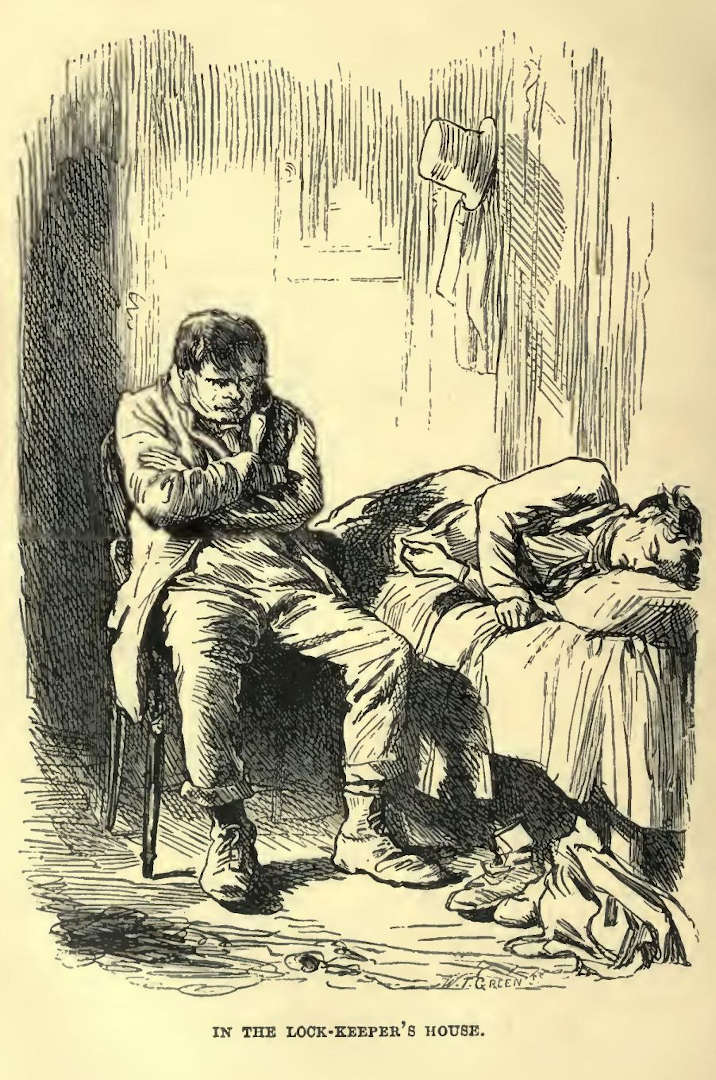
\includegraphics[scale=2.3]{04-01-01}

‘He sleeps sound,’ he said within himself; ‘yet he’s that up to me and
that noticing of me that my getting out of my chair may wake him, when a
rattling peal won’t; let alone my touching of him.’

He very cautiously rose to his feet. ‘T’otherest,’ he said, in a low,
calm voice, ‘are you a lying easy? There’s a chill in the air, governor.
Shall I put a coat over you?’

No answer.

‘That’s about what it is a’ready, you see,’ muttered Riderhood in a
lower and a different voice; ‘a coat over you, a coat over you!’

The sleeper moving an arm, he sat down again in his chair, and feigned
to watch the storm from the window. It was a grand spectacle, but not so
grand as to keep his eyes, for half a minute together, from stealing a
look at the man upon the bed.

It was at the concealed throat of the sleeper that Riderhood so often
looked so curiously, until the sleep seemed to deepen into the stupor
of the dead-tired in mind and body. Then, Riderhood came from the window
cautiously, and stood by the bed.

‘Poor man!’ he murmured in a low tone, with a crafty face, and a very
watchful eye and ready foot, lest he should start up; ‘this here coat
of his must make him uneasy in his sleep. Shall I loosen it for him,
and make him more comfortable? Ah! I think I ought to do it, poor man. I
think I will.’

He touched the first button with a very cautious hand, and a step
backward. But, the sleeper remaining in profound unconsciousness, he
touched the other buttons with a more assured hand, and perhaps the more
lightly on that account. Softly and slowly, he opened the coat and drew
it back.

The draggling ends of a bright-red neckerchief were then disclosed, and
he had even been at the pains of dipping parts of it in some liquid,
to give it the appearance of having become stained by wear. With a
much-perplexed face, Riderhood looked from it to the sleeper, and from
the sleeper to it, and finally crept back to his chair, and there, with
his hand to his chin, sat long in a brown study, looking at both.




\part{Take Note!}
\thispagestyle{plain}

\chapter*{Bibliography}

\bibliography{bib}{}
\bibliographystyle{apalikerd}

\chapter*{Disclaimer}

\section*{Open Access}

The Grounded Theory Review is an open-access journal.
It means 
--- by the international Budapest Open Access Initiative 
\href{https://www.budapestopenaccessinitiative.org/}{(BOAI)}
definition --- that all content is freely available without charge to the user or their institution.
Users can read, download, copy, distribute, print, search, or link texts of this journal fully without asking prior permission from the publisher or the author.



% %%%%%%%%%%%%%%%%
\end{document}%%%%
% End of document.
% %%%%%%%%%%%%%%%%

